\section{Memory consistency}

\label{sec:conc:consistency}

Single-threaded programs have a relatively simple sequential model: instructions
are executed in the order they appear in the source code, subject to the control
flow defined by the programming language.  However, this simple model does not
describe how the program is ultimately executed in most computer architectures.

While it is true that the \emph{effect} of the program is \emph{as if} execution
had proceeded in that manner, compilers and processors are free to carry out
instructions in any way that produces a result indistinguishable from what would
be produced strictly under that model (usually called the \textit{as-if rule},
v. \cite{cppref_asif}).  As the discrepancy between processor and memory access
speeds became increasingly larger under \textit{Moore's law}, hardware designers
started incorporating more complex mechanisms to hide the long latency of memory
operations, and source code became increasingly abstracted from the actual
sequence of operations performed by the machine.

For single-threaded programs, this fact is barely observable in most respects.
Other than secondary effects such as differences in execution time, by
definition the as-if rule does not perturb their execution.  However, as Moore's
law began to falter, increasingly performance improvements are achieved by the
use of additional processor cores, instead of the previous regular increase in
transistor count.  This has made understanding and managing the compiler and
hardware transformations a critical factor in writing correct and efficient
software.

When multiple threads of execution are involved, a \textit{memory model} must be
defined to govern the interaction of different threads observing and mutating
the same region of memory.  The memory system itself is effectively atomic, from
the perspective of the execution threads, making the models serializable.  The
two aspects of a memory model are:

\begin{description}
    \item[Memory coherence]
        constrains the observable behavior of reads and writes to the
        \emph{same} memory location.  Operations can be thought of as occurring
        in a single timeline and all processors agree on that order.  No
        constraint is imposed on the \emph{order} of the operations, only on the
        coherence across processors.
    \item[Memory consistency]
        constrains the observable behavior of reads and writes to
        \emph{different} memory locations with respect to each other and other
        instructions.
\end{description}

The four orderings governed by a memory consistency model are:

\begin{description}
    \item[W $\to$ R] write must complete before subsequent read
    \item[R $\to$ R] read must complete before subsequent read
    \item[R $\to$ W] read must complete before subsequent write
    \item[W $\to$ W] write must complete before subsequent write
\end{description}

As will be discussed in the next sections, different components, from the
compiler to the processors to the memory system, can affect these orderings.  In
general, when analyzing source code, a change made by any of them is equivalent
to any other such that they can be referred to and described as simple
reorderings at the source level.

\subsection{Sequential consistency (SC)}

A \textit{sequentially consistent} memory model (\cite{Lamport1979}) maintains
all four memory operation orderings --- the \textit{program order} of loads and
stores.  In a sequentially consistent model, the following program (where
\texttt{a} and \texttt{b} are global variables initially set to \texttt{0}) will
output either \texttt{01} or \texttt{11}, but never \texttt{00} or \texttt{10}.

\begin{center}
    \begin{tabular}{rl}
        \begin{lstlisting}[style=c]
// thread 0
a = 1;
printf("%d", b);
        \end{lstlisting}
        &
        \begin{lstlisting}[style=c]
// thread 1
b = 1;
printf("%d", a);
        \end{lstlisting} \\[1.5em]
    \end{tabular}
\end{center}

This can be demonstrated by exhaustively listing all the possible ways in which
the four statements can be interleaved (figure \ref{fig:conc:seq}).  To simplify
the notation, we use \texttt{a = b = 1} to denote the state where both stores
happened before the loads, and \texttt{p0}/\texttt{p1} as shorthand for the
\texttt{printf} in each thread.

\begin{figure}[ht]
    \centering
    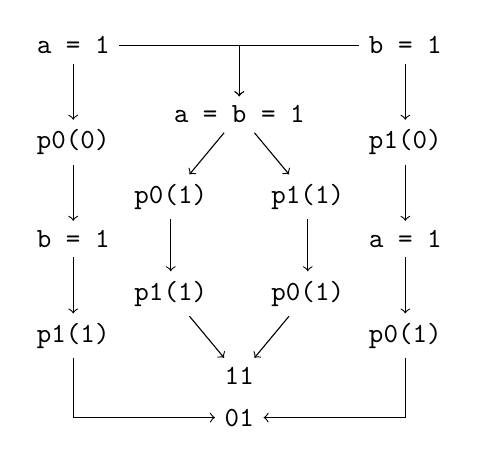
\begin{tikzpicture}[font = \ttfamily, node distance = 3.5em]
        \def\align#1#2{($ (0, 0)!#1!(1, 0) + (0, 0)!#2!(0, 1) $)}
        \node (start) {};
        \node (a1)   [ left of = start, xshift = -2.5em] {a = 1};
        \node (b1)   [right of = start, xshift = +2.5em] {b = 1};
        \node (t0_0) [below of =   a1] {p0(0)};
        \node (t1_0) [below of =   b1] {p1(0)};
        \node (t1_1) [below of = t1_0] {a = 1};
        \node (t0_1) [below of = t0_0] {b = 1};
        \node (t0_2) [below of = t0_1] {p1(1)};
        \node (t1_2) [below of = t1_1] {p0(1)};
        \node (a1b1) [below of = start, yshift = 1em] {a = b = 1};
        \node (c0_0) [below  left of = a1b1, yshift = -0.5em] {p0(1)};
        \node (c1_0) [below right of = a1b1, yshift = -0.5em] {p1(1)};
        \node (c0_1) [below of = c0_0] {p1(1)};
        \node (c1_1) [below of = c1_0] {p0(1)};
        \node (o11)  [below right of = c0_1, yshift = -0.5em] {11};
        \node (o01)  [below of = o11, yshift = 2em] {01};
        \path[->] (a1) edge (t0_0) (t0_0) edge (t0_1) (t0_1) edge (t0_2);
        \path[->] (b1) edge (t1_0) (t1_0) edge (t1_1) (t1_1) edge (t1_2);
        \draw[->] (a1) -| (a1b1);
        \draw[->] (b1) -| (a1b1);
        \path[->] (a1b1) edge (c0_0) (c0_0) edge (c0_1);
        \path[->] (a1b1) edge (c1_0) (c1_0) edge (c1_1);
        \path[->] (c0_1) edge (o11);
        \path[->] (c1_1) edge (o11);
        \draw[->] (t0_2) |- (o01);
        \draw[->] (t1_2) |- (o01);
    \end{tikzpicture}
    \caption{Sequentially consistent execution graph}
    \label{fig:conc:seq}
\end{figure}

This graph shows all four possible execution paths (with only two being
externally distinguishable), which are much less than the $4! = 24$ permutations
of the four initial statements.  The strict sequentially consistent model
establishes \textit{happens before} relations (\cite{Lamport1978}) between every
operation in a single thread, which can be seen in the graph as there are no
edges that go from an operation to another that precedes it in the same thread.
Thus, there are only two options: either one thread executes entirely before the
other (in which case the output is \texttt{01}) or both stores happen followed
by both loads (in which case the output is \texttt{11}).

Far from trivial, figure \ref{fig:conc:dekker_peterson} shows that the same
reasoning can be applied to solve a very important concurrent problem: mutual
exclusion\footnotemark.  The loads and stores in this program are analogous to
the ones in the previous execution graph.  They can be analyzed in terms of the
outputs described before:

\footnotetext{
    The code in this listing is a simplification of \textit{Dekker's} and
    \textit{Peterson's} algorithms.  It is only concerned with mutual exclusion
    and is enough to demonstrate the effects of memory consistency.  Those
    algorithms also handle contention and more than two processes and avoid
    starvation.}

\begin{figure}
    \centering
    \begin{tabular}{cc}
        \begin{lstlisting}[style=c]
bool flag0 = false;

void t0(void) {
    flag0 = true;
    if(flag1) {
        // contended
    } else {
        // critical section
        flag0 = false;
    }
}
        \end{lstlisting}
        &
        \begin{lstlisting}[style=c]
bool flag1 = false;

void t1(void) {
    flag1 = true;
    if(flag0) {
        // contended
    } else {
        // critical section
        flag0 = false;
    }
}
        \end{lstlisting}
    \end{tabular}
    \caption{Simplified Dekker's/Peterson's algorithm}
    \label{fig:conc:dekker_peterson}
\end{figure}

\begin{itemize}
    \item
        \texttt{00}: both processes see the flags as not set and enter the
        critical section.  Impossible by the rules of sequential consistency.
    \item
        \texttt{01}: a process sees one of the flags unset and enters the
        critical section.  The other process sees the other flag set and does
        not.  This is the desired outcome.
    \item
        \texttt{10}: a process sees one of the flags set without the other
        subsequently seeing the other flag set.  Harmless, but also impossible
        in a sequentially consistent model.
    \item
        \texttt{11}: both processes observe the flags as set.  None enters the
        critical section.
\end{itemize}

From these rules, it can be determined that mutual exclusion is guaranteed under
the rules of the sequential consistency model.  Sequential consistency is an
intuitive and convenient model as it closely follows source code order.  For
this reason, it is the preferred model of many programming languages
(\textit{sequentially consistent for data-race-free programs}, SC-DRF).
Maintaining sequential consistency, however, effectively serializes computation,
negating all benefits of instruction- and thread-level parallelism.  For this
reason, no modern processor is fully sequentially consistent, as the
synchronization cost would be prohibitive.

Most systems offer one of the many \textit{relaxed memory consistency} models,
allowing certain orderings to be violated.  Each relaxation gives the hardware
more freedom in how it can process instructions and service memory requests.  A
model that is more relaxed than sequential consistency commonly offers
\textit{barrier} (or \textit{fence}) instructions to effectively reinstate
sequential consistency at particular points in a program.  A barrier forces some
or all preceding memory operations to complete before some or all subsequent
memory operations can start.  These instructions are added only to the critical
areas where inter-processor communication and synchronization is required,
allowing the rest of the program to benefit from the many aforementioned
hardware optimizations.

\subsection{Total Store Ordering (TSO)}

Relaxing the W $\to$ R ordering allows an independent read to be issued before a
write completes.  A store often must wait for an acknowledgment message from
another CPU (v. \secrefpar{sec:conc:coherence}), which can take up to hundreds
of cycles, so this can eliminate long stalls in the pipeline.  It is a crucial
transformation as loads usually occur at a much higher rate and are much less
expensive to perform than stores, which require processor synchronization and
flushing of caches to main memory.  It is often the most important and common
relaxation in a memory model.

A \textit{write buffer} (or \textit{store buffer}) in each processor can be used
to allow reads to proceed while prior writes are executed.  Stores are placed in
the buffer and subsequent loads are executed immediately.  Further writes are
enqueued on the write buffer (i.e. there is no W $\to$ W reordering).  From the
point of view of the program, several instructions are now executed in
parallel\footnotemark.  This is a different type of parallelism than separate
threads being executed by multiple cores.  In this scenario, called
\textit{instruction-level parallelism} (ILP), several instructions in a single
instruction stream are executed in parallel.

\footnotetext{
    Of course, as described in the introduction of this section, the behavior
    described in this section is not directly visible to a well-behaved program.
    Nonetheless, they are indirectly observable.  The program can, for example,
    measure that the execution of a sequence of instructions was done in less
    cycles than their combined cycle count.  This is one reason why performance
    analysis and prediction in modern processors is difficult.}

The \textit{x86/64} architecture and its \textit{Total Store Ordering} model are
an example of this relaxation.  Synchronization instructions are required for
instruction ordering not guaranteed by the model:

\begin{description}
    \item[\texttt{lfence}] waits for all loads to complete
    \item[\texttt{sfence}] waits for all stores to complete
    \item[\texttt{mfence}] waits for all operations to complete
\end{description}

Even this single relaxation in the ordering of memory operations has profound
consequences.  Consider for example how the delay in the propagation of writes
due to a store buffer affects the mutual exclusion example in the previous
section.  Barrier instructions now would have to be inserted to reinstate the
sequentially consistent model to preserve the original order of operations.
In general, any code in the form:

\begin{center}
    \begin{tabular}{cc}
        \begin{lstlisting}[style=c]
// thread0
a = 1;
b = 1;
        \end{lstlisting}
        &
        \begin{lstlisting}[style=c]
// thread1
if(b)
    assert(a);
        \end{lstlisting}
    \end{tabular}
\end{center}

will not work as expected in the presence of a store buffer.  The reason for
this is \texttt{b} might be already in the CPU's cache while \texttt{a} is not.
The difference in propagation of stores could cause the other CPU to see them in
the reverse order.  The general solution is to add a memory barrier:

\begin{center}
    \begin{tabular}{cc}
        \begin{lstlisting}[style=c]
// thread0
a = 1;
_mm_mfence();
b = 1;
        \end{lstlisting}
        &
        \begin{lstlisting}[style=c,showlines=true]
// thread1
if(b)
    assert(a);

        \end{lstlisting}
    \end{tabular}
\end{center}

Upon executing the barrier instruction, the CPU will be prevented from
transmitting further stores until all previous stores have been acknowledged and
completed.  This ensures \texttt{thread1} does not see the store to \texttt{b}
before the store to \texttt{a}, thus preserving program order.  It is not,
however, quite sufficient to ensure the correctness of the program.  The reason
for this is another component associated with the store buffer, the
\textit{invalidate queue}.

A CPU which receives a request to remove a line from its cache can take a long
time to respond if the cache is busy (e.g. when several \emph{invalidate}
messages arrive in a short period, as can happen immediately following a memory
barrier if a CPU is executing many stores).  The addition of an invalidate queue
is based on the fact that responding to the request does not have to wait for
the actual removal from the cache: as long as the CPU maintains internal
consistency, it can respond immediately and place the invalidation in the queue,
to be executed at a later time.

In the previous example, \texttt{thread1}'s immediate invalidation
acknowledgement of \texttt{a} can cause \texttt{thread0} to progress past its
memory barrier and execute the store to \texttt{b}.  If \texttt{thread1} then
receives the new value of \texttt{b} before processing the invalidation of
\texttt{a}, it could still perceive the two stores in the opposite order.
Therefore, a \emph{second} memory barrier is needed:

\begin{center}
    \begin{tabular}{cc}
        \begin{lstlisting}[style=c,showlines=true]
// thread0
a = 1;
_mm_mfence();
b = 1;

        \end{lstlisting}
        &
        \begin{lstlisting}[style=c]
// thread1
if(b) {
    _mm_mfence();
    assert(a);
}
        \end{lstlisting}
    \end{tabular}
\end{center}

Note, however, that only the store buffer is of concern in \texttt{thread0} (the
writer) and only the invalidate queue is of concern in \texttt{thread1} (the
reader).  There is no reason to affect the other component in each of the
threads.  For cases like this, which are very common, certain architectures
provide specialized barrier instructions:

\begin{center}
    \begin{tabular}{cc}
        \begin{lstlisting}[style=c,showlines=true]
// thread0
a = 1;
_mm_sfence();
b = 1;

        \end{lstlisting}
        &
        \begin{lstlisting}[style=c]
// thread1
if(b) {
    _mm_lfence();
    assert(a);
}
        \end{lstlisting}
    \end{tabular}
\end{center}

The \emph{store} and \emph{load} fences will (roughly speaking) only operate on
the store buffer and invalidate queue, respectively, allowing the other
component to operate without restrictions.

\subsection{Processor Consistency (PC)}

Relaxing the W $\to$ W ordering allows various transformations of memory stores
with respect to each other.  The \textit{SPARC} architecture is an example of
this relaxation which allows write coalescing in the write buffer when they
share the same cache line, saving memory bandwidth due to the reduced number of
stores, or complete reordering of memory stores.  Its \textit{Processor
Consistency} model further differs from TSO in that \emph{any} processor can
read the new value in a memory location before the store is observed by all
processors, while in TSO reads by other processors cannot return the new value
until the store is observed by \emph{all} processors.

The simple program below demonstrates the difference between these two models.
Under TSO, thread 2 cannot observe the write to \texttt{b} before the write to
\texttt{a}.  Under PC, however, there is no dependency between the two stores,
so thread 2 may see the write to \texttt{b} before the write to \texttt{a}.
Note that even the addition of a memory barrier in \texttt{thread1} would not
guarantee correctness, since barriers only affect a given CPU's view of memory,
i.e. there is no transitivity relation across CPUs.

\begin{center}
    \begin{tabular}{ccc}
        \begin{lstlisting}[style=c,showlines=true]
// thread 0
a = 1;

        \end{lstlisting}
        &
        \begin{lstlisting}[style=c]
// thread 1
while(!a);
b = 1;
        \end{lstlisting}
        &
        \begin{lstlisting}[style=c]
// thread 2
while(!b);
printf("%d", a);
        \end{lstlisting}
    \end{tabular}
\end{center}

\textit{Partial Store Ordering} (PSO) is a more extreme relaxation of the same
ordering, which allows complete reordering of memory stores.  The following
program would not match sequential consistency in this model, as there is no
guaranteed order for the two stores in thread 0:

\begin{center}
    \begin{tabular}{cc}
        \begin{lstlisting}[style=c]
// thread 0
a = 1;
flag = 1;
        \end{lstlisting}
        &
        \begin{lstlisting}[style=c]
// thread 1
while(!flag);
printf("%d", a);
        \end{lstlisting}
    \end{tabular}
\end{center}

\subsection{Weak Ordering (WO), Release Consistency, (RC)}

Weak ordering memory models\footnotemark allow all four types of operation
reordering.  \textit{Weak Ordering} and \textit{Release Consistency} are
examples of this type of model, one based on fences and the other on
acquire/release semantics.  \textit{ARM} and \textit{PowerPC} are examples of
architectures with very relaxed consistency models.

\footnotetext{
    ``Weak ordering'' is sometimes used \textit{lato sensu} to refer to all
    models which are more relaxed than sequential consistency.  The term is
    always used \textit{stricto sensu} here.}
